\documentclass[../main.tex]{subfiles}
\graphicspath{{\subfix{../images/}}}
\begin{document}

\begin{definition}


    Neorientovaný prostý graf $\mathbb{G} = (\mathbb{V}, \mathbb{E})$ \\
    $\mathbb{V}$ konečná množina vrcholů \\
    $\mathbb{E} \subseteqq \binom{V}{2}$ \\
    $\mathbb{E} $ množina hran\\
    $\binom{V}{2}$  množina všech neuspořádaných dvojic z $\mathbb{V}$ \\


    Často $|\mathbb{V}|=n$,\\
    často $\mathbb{V} = [n]$, kde $[n] = \{1,2,...,n\}$ 
\end{definition}


\begin{definition}
    Nechť $\mathbb{G} = (\mathbb{V}, \mathbb{E})$, pak definujeme \\
    $\mathbb{E}(\mathbb{G}) = \mathbb{E}$\\
    $\mathbb{V}(\mathbb{G}) = \mathbb{V}$
\end{definition}

\begin{definition}
    Pro graf $\mathbb{G} = (\mathbb{V}, \mathbb{E})$ definujme  doplněk $\mathbb{G} \coloneq \bar{\mathbb{G}}$ je graf $(V, \binom{V}{2}\setminus E )$
\end{definition}

\begin{definition}
    Nulový graf $G = (\emptyset, \emptyset)$ 
\end{definition}

\begin{example}
    Kolik je různých grafů na $[n]$?

    \begin{figure}[h]
        \centering
        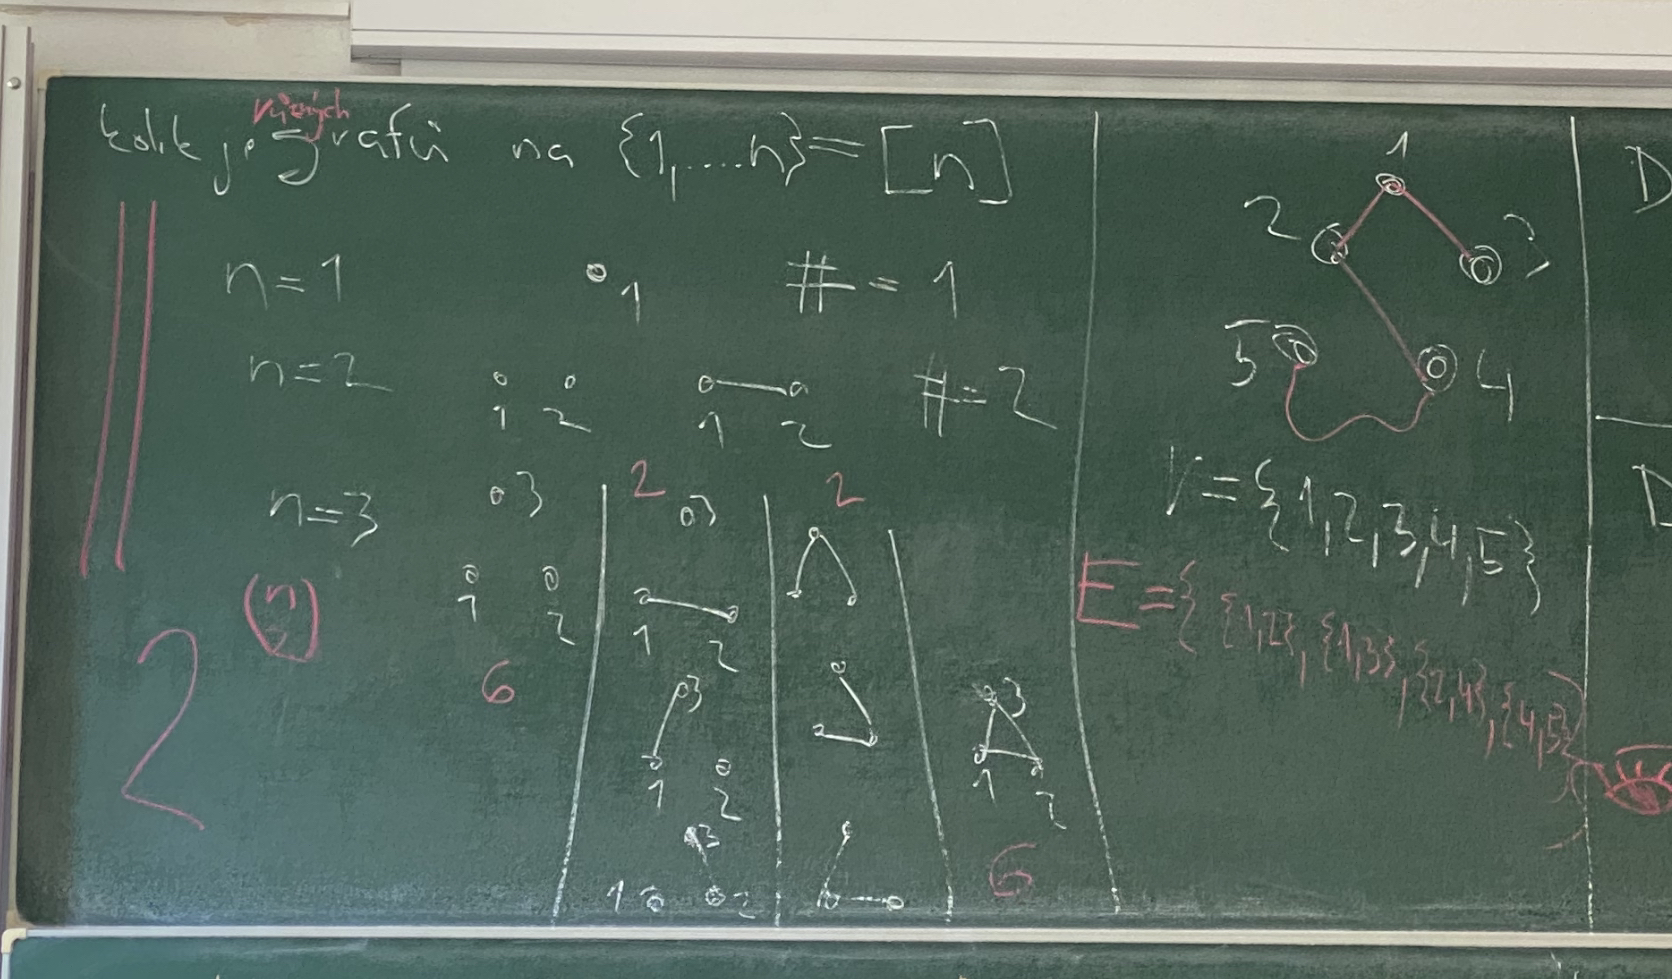
\includegraphics[width=\textwidth/2]{images/27-9-pocetgrafu.png}
        \caption*{Na obrázku vidíme různý počet grafů}
    \end{figure} 

    Poté co se zamyslíme tak vidíme, že jich je obecně $2^{\binom{n}{2}}$
\end{example}



\begin{definition}
    $\mathbb{G} = (\mathbb{V}, \mathbb{E})$ a $\mathbb{H} = (\mathbb{W}, \mathbb{F})$ jsou isomorfní, jestliže existuje bijekce 
    $f: V \mapsto W, (|V| = |W|)$ tak, že $\forall u,v \in V: \{u, v\}\in E \Leftrightarrow \{ f(u), f(v) \} \in F$
\end{definition}


\begin{definition}
    $f$ je automorfismus jestliže jde o isomorfismus mezi $G$ a $G$ 
\end{definition}

\begin{remark}
    $Aut(G) = \{f | f\text{ je automorfismus }G\}$ je grupa
\end{remark}


\begin{example}
    Kolik je navzájem neisomorfních grafů s n vrcholy?

    \begin{figure}[h]
        \centering        
        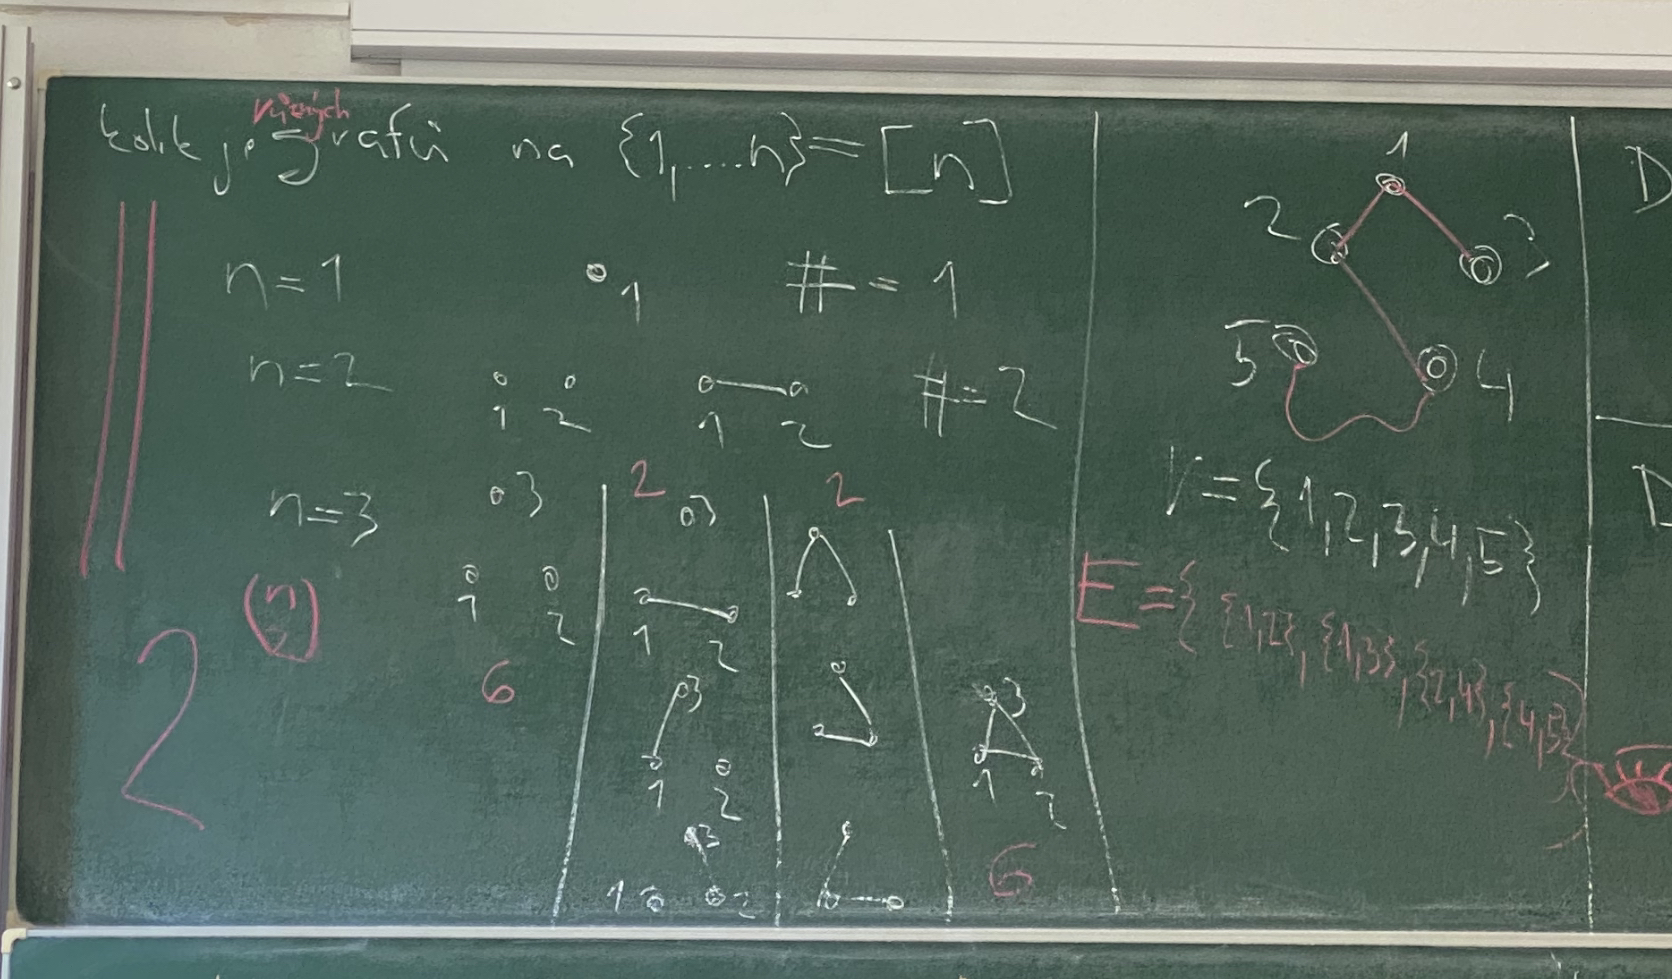
\includegraphics[width=\textwidth/2]{images/27-9-pocetgrafu.png}
        \caption*{Každá "kategorie" grafů je jeden isomorfismus}
    \end{figure} 

    Není vzorec, musí se počítat, existují horní a dolní odhady.
\end{example}

\begin{claim}
Dolní odhad počtu navzájem neisomorfních grafů s n vrcholy je alespoň
\begin{equation}
    \frac{2^{\binom{n}{2}}}{n!} \geq \frac{2^{\binom{n}{2}}}{n^n} \approx \frac{2^{\frac{n^2}{2}}}{2^{n \log(n)}} \approx 2^{(\frac{1}{2} - \varepsilon)n^2} 
\end{equation}
\end{claim}

\begin{proof}
    Označme $g_n$ jako množinu všech neisomorfních grafů na [n]
    \begin{equation*}
        2^{\binom{n}{2}} = \sum_{g_n} \frac{n!}{|Aut(G)|} \leq n! |g_n|
    \end{equation*}

\end{proof}

\begin{claim}
    (Bez důkazu)

    $\forall\varepsilon>0 \exists n_0 \forall n\geq n_0$

    $|g_n|\leq (1+\varepsilon) \frac{2^{\binom{n}{2}}}{n!}$
\end{claim}


\begin{definition}
    Pro graf $\mathbb{G} = (\mathbb{V}, \mathbb{E})$ a vrchol $v\in V$ Označme

    $N_G (v) \coloneq \left\{ x\in V: \{x, v\} \in E \right\}$, prvkům říkáme sousedé $v$ 

    $|N_G (v)| = deg_G(v)$, stupeň
\end{definition}


\begin{claim}
    $\sum_{v\in V} deg (v)$ je sudé číslo
\end{claim}
\begin{proof}
    $\sum_{v\in V} deg (v) = 2|E|$
\end{proof}

\begin{definition}
    $\mathbb{G} = (\mathbb{V}, \mathbb{E})$ graf, $v\in V, e\in E$: $v$ je incidentní s $e$, jestliže $s\in e$

    $e\in E, f\in E$, $e$ je incidentní s $f$ jestliže $|e\cap f| = 1$
\end{definition}


\begin{definition}
    Sled v grafu G

    Alternující posloupnost vrcholů a hran, např $v_0, e_1, v_1, e_2, v_2 ......... e_k v_k$ 
\end{definition}

\begin{definition}
    tah v grafu G, sled $\forall i\neq j \implies e_i \neq e_j$
\end{definition}

\begin{definition}
    cesta v G, sled $\forall i\neq j \implies v_i \neq v_j$

\end{definition}



\begin{definition}
    sled v G je z $u$ do $w$ jestliže $\exists$ sled, $u = v_0 e_1 .... e_k v_k = w$

    Cesta v G je z $u$ do $w$ jestliže $\exists$ sled z $u$ do $w$ tak že se žádný vrchol nevyskytuje dvakrát.
\end{definition}


\begin{claim}
    Buď $G=(V,E)$ graf a $u,w\in V$ jeho dva vrcholy. Následující dvě tvrzení jsou potom ekvivalentní.

    \begin{enumerate}
        \item Existuje sled v $G$ z vrcholu $u$ do $w$
        \item Existuje cesta v $G$ z vrcholu $u$ do $w$
    \end{enumerate}
\end{claim}

\end{document}